\documentclass[10pt,a4paper]{article}

% ---------- Packages ----------
\usepackage[a4paper,margin=1.5cm,headheight=14pt]{geometry}
\usepackage[T1]{fontenc}
\usepackage{lmodern}
\usepackage{microtype}
\usepackage{graphicx}
\usepackage{amsmath}
\usepackage{booktabs}
\usepackage{tabularx}
\usepackage{array}
\usepackage{xcolor}
\usepackage{enumitem}
\usepackage{fancyhdr}
\usepackage{titlesec}
\usepackage{hyperref}
\usepackage{tcolorbox}

% ---------- Colours ----------
\definecolor{navy}{HTML}{17324D}
\definecolor{teal}{HTML}{176B87}
\definecolor{lightblue}{HTML}{EAF4F7}
\definecolor{borderblue}{HTML}{B8DDE8}
\definecolor{greytext}{HTML}{486581}

% ---------- Hyperlinks ----------
\hypersetup{
    colorlinks=true,
    linkcolor=teal,
    urlcolor=teal,
    citecolor=teal
}

% ---------- Page Style ----------
\pagestyle{fancy}
\fancyhf{}
\fancyfoot[L]{\footnotesize\color{greytext} Camera-Driven Mobile Robot Digital Twin}
\fancyfoot[R]{\footnotesize\color{greytext}\thepage}
\renewcommand{\headrulewidth}{0pt}
\renewcommand{\footrulewidth}{0.4pt}

% ---------- Section Formatting ----------
\titleformat{\section}
  {\large\bfseries\color{teal}}
  {}{0pt}{}
  [\vspace{-2pt}\color{borderblue}\titlerule]

\titleformat{\subsection}
  {\normalsize\bfseries\color{navy}}
  {}{0pt}{}

\titlespacing*{\section}{0pt}{4pt}{2pt}
\titlespacing*{\subsection}{0pt}{3pt}{1pt}

% ---------- Paragraph Formatting ----------
\setlength{\parindent}{0pt}
\setlength{\parskip}{2pt}
\setlist[itemize]{
    leftmargin=1.2em,
    itemsep=1pt,
    topsep=1pt
}
\setlist[enumerate]{
    leftmargin=1.2em,
    itemsep=1pt,
    topsep=1pt
}

\renewcommand{\arraystretch}{1.06}

\begin{document}

% ==========================================================
% TITLE
% ==========================================================

\begin{center}
    {\LARGE\bfseries\color{navy}
    Camera-Driven Mobile Robot Digital Twin}

    \vspace{2pt}

    {\small\color{greytext}
    Physical Object Tracking and Real-Time Obstacle Synchronisation in CoppeliaSim}
\end{center}

\vspace{-4pt}

% ==========================================================
% SUMMARY BOX
% ==========================================================

\begin{tcolorbox}[
    colback=lightblue,
    colframe=borderblue,
    boxrule=0.6pt,
    arc=1.5mm,
    left=6pt,
    right=6pt,
    top=3pt,
    bottom=3pt
]
\begin{minipage}[t]{0.48\linewidth}
\textbf{\color{navy}Objective}

Demonstrate an integrated physical-to-virtual loop connecting a real-world desktop observation area to an autonomous mobile robot simulation in CoppeliaSim.
\end{minipage}
\hfill
\begin{minipage}[t]{0.48\linewidth}
\textbf{\color{navy}Current Implementation (v1)}

Real-time 2D camera tracking (ArUco / HSV color), spatial coordinate mapping, ZeroMQ simulation synchronisation, and reactive Pioneer P3DX obstacle avoidance.
\end{minipage}
\end{tcolorbox}

\vspace{-4pt}

% ==========================================================
\section{System Overview}
% ==========================================================

This technical report details the implementation of a real-time digital twin connecting a physical desktop camera feed to the \textbf{CoppeliaSim} robotics simulator. A standard webcam monitors a defined desk workspace, tracking a physical marker or colored object. The estimated physical coordinates are mapped into a $3.0\,\mathrm{m}\times3.0\,\mathrm{m}$ virtual arena, updating the position of a simulated cylindrical obstacle in real time.

Inside the simulation, an autonomous \textbf{Pioneer P3DX} mobile robot navigates along a perimeter patrol route. When the physical obstacle is moved into the robot's forward path, the robot detects the obstruction and halts safely. Once the obstacle is cleared from the path, the robot automatically resumes its navigation loop.

\vspace{1pt}
\begin{center}
    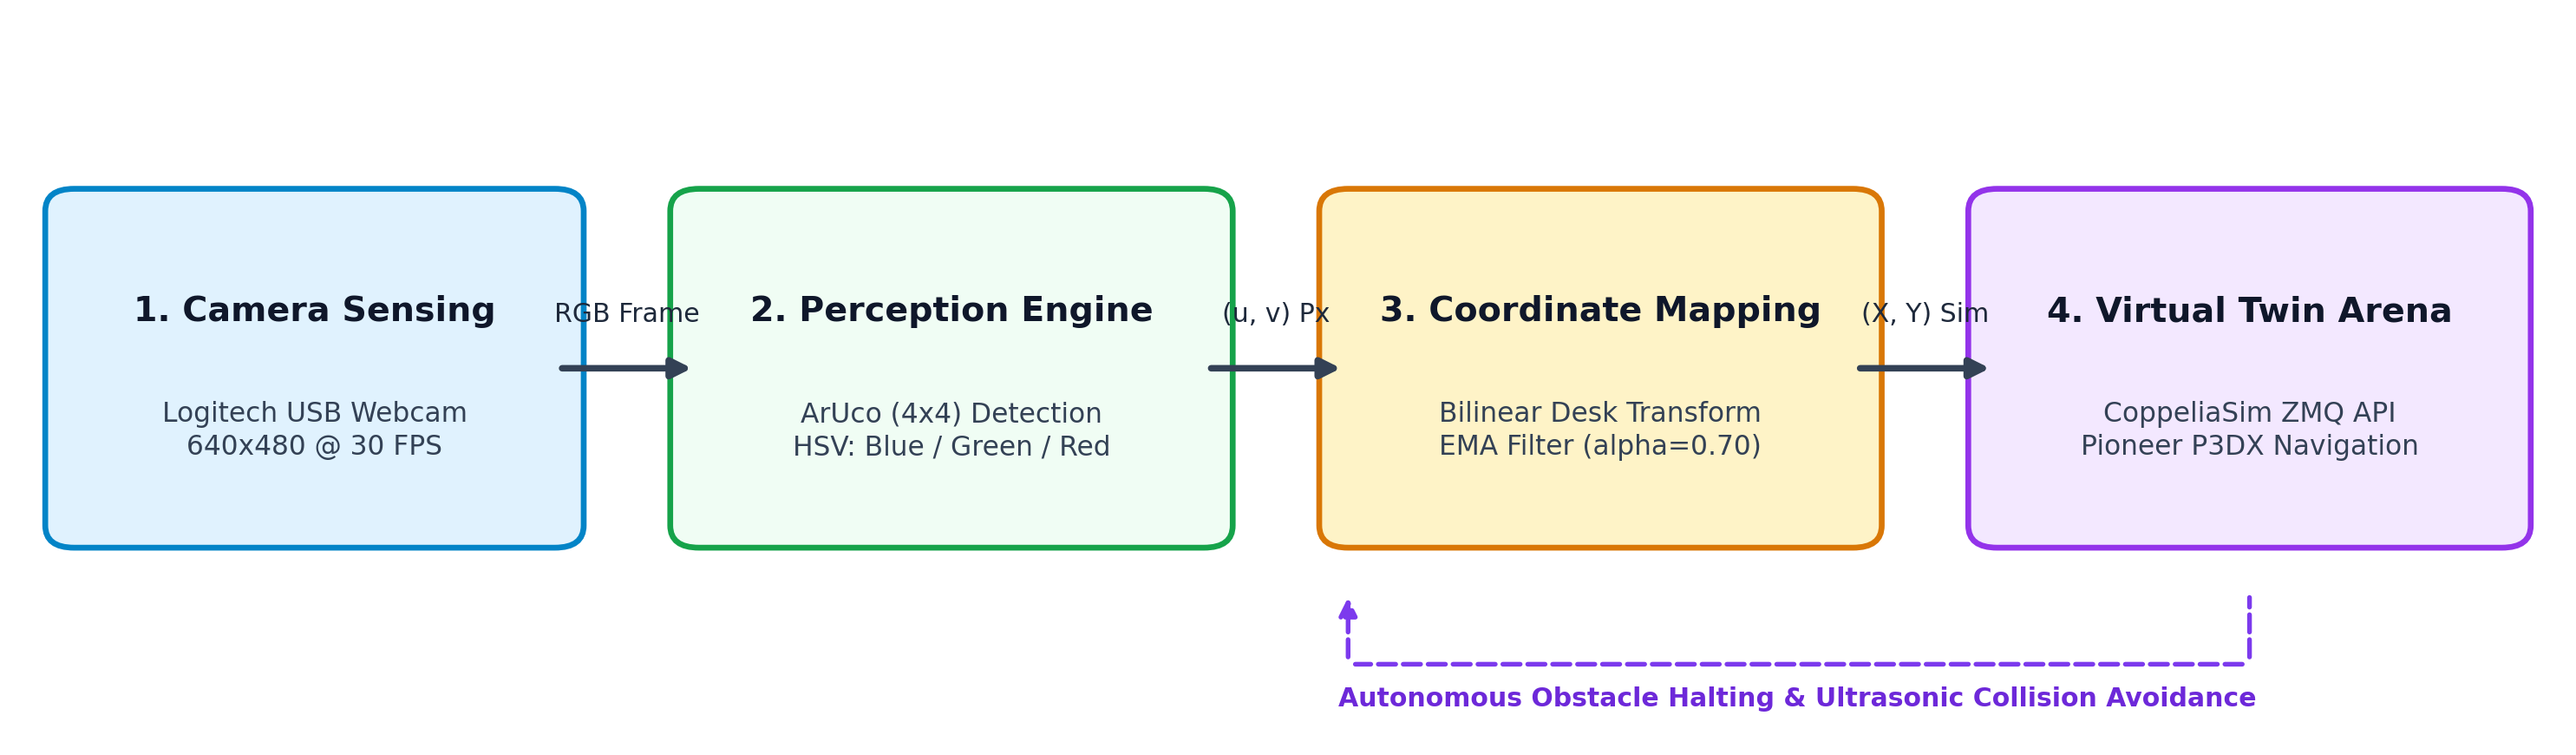
\includegraphics[width=0.97\linewidth]{report_assets/fig_architecture.png}\\[-3pt]
    \footnotesize\color{greytext}\itshape
    Figure 1. Data pipeline: real-world camera tracking updates the virtual obstacle in CoppeliaSim to govern simulated robot navigation.
\end{center}
\vspace{-4pt}

% ==========================================================
\section{Technical Implementation}
% ==========================================================

The system operates across four coordinated stages:

\begin{itemize}
    \item \textbf{Vision and Perception:} An overhead webcam captures $640\times480$ RGB frames at 30 FPS. OpenCV provides two practical tracking modes without requiring neural network dependencies:
    \begin{itemize}
        \item \textit{ArUco Marker Tracking:} Detects \texttt{DICT\_4X4\_50} markers and computes the centroid $(c_u, c_v)$ from the four marker corners, providing reliable tracking across varying room illumination.
        \item \textit{HSV Color Segmentation:} Provides calibrated presets for Red, Green, and Blue objects. Morphological opening and closing operations filter background noise, and spatial moments ($c_u = M_{10}/M_{00},\; c_v = M_{01}/M_{00}$) determine the object center.
    \end{itemize}

    \item \textbf{Spatial Coordinate Mapping:} Pixel coordinates within a calibrated desk Region of Interest (ROI: $[100, 540]\times[60, 420]\,\mathrm{px}$) are normalized and linearly transformed to arena coordinates $(X_{\text{sim}}, Y_{\text{sim}}) \in [-1.4\,\mathrm{m}, +1.4\,\mathrm{m}]$. An Exponential Moving Average (EMA) filter ($\alpha = 0.70$) smooths hand tremor during physical adjustments:
    \begin{equation}
        \mathbf{p}_{\text{smooth}}[t] = \alpha \cdot \mathbf{p}_{\text{raw}}[t] + (1 - \alpha) \cdot \mathbf{p}_{\text{smooth}}[t-1]
    \end{equation}
    A state watchdog holds the last known position for $2.0\,\mathrm{s}$ if tracking is briefly occluded, preventing abrupt simulation jumps.

    \item \textbf{Simulation Interface:} Communication with CoppeliaSim is handled via the ZeroMQ Remote API (port 23000). The script updates the obstacle position in the 3D scene and retrieves robot odometry and ultrasonic sensor readings at low latency ($<15\,\mathrm{ms}$).

    \item \textbf{Pioneer P3DX Navigation \& Safety Halting:} The robot follows a perimeter route around four corner waypoints ($\pm 0.95\,\mathrm{m}, \pm 0.95\,\mathrm{m}$) at a cruising speed of $0.16\,\mathrm{m/s}$. When arriving within $0.16\,\mathrm{m}$ of a waypoint, the robot halts forward motion and turns in place ($\omega = 0.60\,\mathrm{rad/s}$) until aligned with the next waypoint, avoiding wide turns near arena walls. The robot continuously checks the obstacle's relative position: if it falls within $0.65\,\mathrm{m}$ inside a forward heading cone of $\pm 50^\circ$, or if front ultrasonic sensors detect an object closer than $0.18\,\mathrm{m}$, the robot halts immediately until the obstacle is removed.
\end{itemize}

\newpage

% ==========================================================
\section{System Operation \& Visual Verification}
% ==========================================================

The physical tracking and simulation environments run concurrently to verify real-time responsiveness and obstacle detection accuracy.

\vspace{1pt}
\noindent
\begin{minipage}[t]{0.485\linewidth}
    \centering
    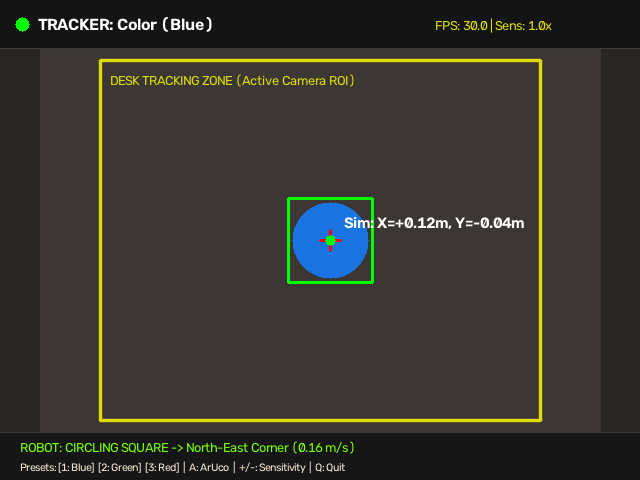
\includegraphics[height=3.4cm, width=\linewidth, keepaspectratio=false]{report_assets/fig_tracking_hud.png}\\[-2pt]
    \footnotesize\textbf{Figure 2:} OpenCV tracking HUD showing desk ROI.
\end{minipage}
\hfill
\begin{minipage}[t]{0.485\linewidth}
    \centering
    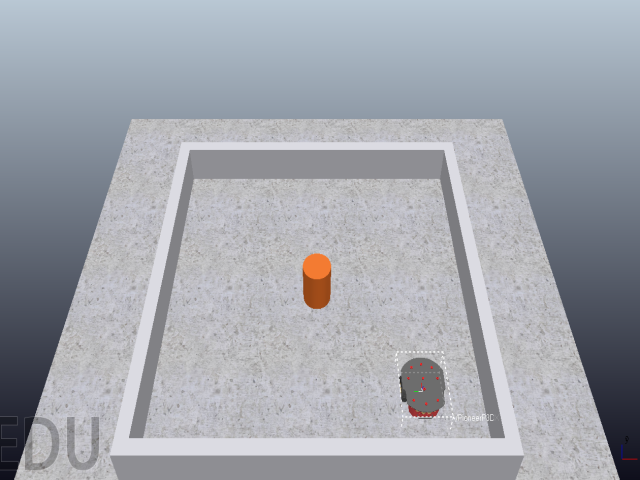
\includegraphics[height=3.4cm, width=\linewidth, keepaspectratio=false]{report_assets/fig_coppelia_twin.png}\\[-2pt]
    \footnotesize\textbf{Figure 3:} Synchronised CoppeliaSim 3D arena.
\end{minipage}
\vspace{1pt}

% ==========================================================
\section{Technical Configuration}
% ==========================================================

\begin{tabularx}{\linewidth}{
    >{\bfseries\color{navy}}p{0.25\linewidth}
    X
}
\toprule
Component & Implementation Details \\
\midrule
Software Stack &
Python 3.10, OpenCV 4.8, CoppeliaSim Edu 4.10, ZeroMQ Remote API, Ubuntu 22.04 LTS \\

Camera Input &
$640\times480$ resolution @ 30 FPS via standard USB webcam and V4L2 backend \\

Object Tracking &
Dual-mode perception: ArUco fiducial detection (\texttt{DICT\_4X4\_50}) and calibrated HSV color presets (Red, Green, Blue) \\

Workspace Mapping &
Desk ROI ($[100, 540]\times[60, 420]\,\mathrm{px}$) mapped to $[-1.4\,\mathrm{m}, +1.4\,\mathrm{m}]$ in virtual arena \\

Position Smoothing &
Exponential Moving Average ($\alpha = 0.70$) with 2.0-second persistence watchdog \\

Robot Navigation &
Differential-drive Pioneer P3DX with waypoint tracking ($v = 0.16\,\mathrm{m/s}$) and in-place corner rotation ($\omega = 0.60\,\mathrm{rad/s}$) \\

Collision Safety &
Forward heading cone safety check ($d < 0.65\,\mathrm{m},\; |\theta| < 50^\circ$) supplemented by simulated frontal ultrasonic sensors ($d < 0.18\,\mathrm{m}$) \\
\bottomrule
\end{tabularx}

% ==========================================================
\section{Significance and Practical Applications}
% ==========================================================

The core contribution of this setup is a responsive physical-to-virtual loop: physical interventions in the real workspace directly modify the simulation and trigger autonomous robot reactions. In practical engineering, this architecture provides a testbed for several real-world digital twin scenarios:

\begin{itemize}
    \item \textbf{Automated Warehouse Logistics (AGVs / AMRs):} In modern fulfillment centers, Autonomous Guided Vehicles must safely navigate dynamic aisles where pallets, carts, and personnel temporarily block designated paths. Connecting overhead facility cameras to a central digital twin enables real-time synchronisation of new obstacles into the navigation model, allowing supervisory systems to verify route viability before robots encounter physical bottlenecks.

    \item \textbf{Industrial Shop Floors and Collaborative Workcells:} In manufacturing environments where human operators work alongside mobile platforms, digital twins provide continuous spatial awareness. Tracking real-world tool carts or materials directly into the virtual twin allows automated verification of safety buffer zones and proactive path halting.

    \item \textbf{Pre-Deployment Navigation Validation:} Testing control algorithms directly on physical mobile robots introduces risks of collision and hardware wear. A camera-driven digital twin allows engineers to physically manipulate obstacles by hand on a test bench to evaluate robot response in complex scenarios prior to deploying code onto physical platforms.
\end{itemize}

% ==========================================================
\section{Future Enhancements}
% ==========================================================

Building on this foundational v1 implementation, planned technical enhancements include:

\begin{itemize}
    \item \textbf{Multi-Sensor Fusion (LiDAR + Camera):} Integrating 2D/3D LiDAR alongside the optical camera to combine dense planar distance measurements with visual feature classification, overcoming occlusion when objects overlap.
    \item \textbf{Multi-Camera Workspace Coverage:} Expanding from a single desk camera to calibrated multi-view camera feeds to eliminate blind spots across larger room-scale tracking zones.
    \item \textbf{Physical Hardware Actuation:} Connecting the virtual navigation planner to a physical Pioneer P3DX or ROS-based mobile robot, completing the bi-directional cycle where simulated planning directly drives physical hardware.
\end{itemize}

\vspace{1pt}

\begin{tcolorbox}[
    colback=lightblue,
    colframe=borderblue,
    boxrule=0.6pt,
    arc=1.5mm,
    left=6pt,
    right=6pt,
    top=2.5pt,
    bottom=2.5pt
]
\small
\textbf{\color{navy}Project Repository and Setup Guide:}
\href{https://github.com/madebyNaveedh/camera-digital-twin}
{\texttt{github.com/madebyNaveedh/camera-digital-twin}}
\end{tcolorbox}

\end{document}
